\documentclass[11pt]{article}
\usepackage{amssymb, amsmath}
\usepackage{amsthm}
\usepackage{url,hyperref}
\usepackage{algorithm}
\usepackage{algpseudocode}
\usepackage[numbered]{mcode}
\usepackage{graphicx}

\topmargin -2cm
\textheight 23cm
\textwidth 6.5in
\oddsidemargin -.1in
\evensidemargin -.1in
\topmargin -1.5cm
\linespread{1.25}

% ----------------------------------------------------------------
% TODO: Enter your name, and your student number, and your topic below
% ----------------------------------------------------------------
\newcommand{\SName}{{Gabriel Luong}}
\newcommand{\SNumber}{{996268275}}
\newcommand{\Topic}{{CSC420 Assignment 1}}
% ----------------------------------------------------------------

\title{\Topic\\
}
\author{
	\SName \\ 
	\SNumber 
	\date{}
}

\begin{document}
\maketitle
%----------------------------------------------------------------
% Question 1
%----------------------------------------------------------------
\section{}

\begin{algorithm}
\caption{Convolution}
\begin{algorithmic}[1]
\Procedure{Convolution}{$Image(i \times j), Filter(u \times v)$}
	\State G $\gets$ new i $\times$ j image matrix
	\For{ImageY = 0 to j}
		\For{ImageX = 0 to i}
			\State sum $\gets$ 0
			\For{FilterY = -v to v}
				\For{FilterX = -u to u}
					\State sum $\gets$ sum + Filter(FilterX, FilterY) $\times$ Image(ImageX + FilterX, ImageY + FilterY)
				\EndFor
			\EndFor
			\State G(ImageX, ImageY) = sum
		\EndFor
	\EndFor
	\State \textbf{return} G
\EndProcedure
\end{algorithmic}
\end{algorithm}

%----------------------------------------------------------------
% Question 2
%----------------------------------------------------------------
\section{}
(a) For a given $n$ x $n$ image, $I$, and $m$ x $m$ filter, $h$, the process of performing a convolution requires $m^2$ operations per pixel in $I$ which results in a time complexity of $O(n^2m^2)$. However, the complexity of convolution with the help of Fourier Transform can be reduced to $O(nlogn)$. If $h$ can be separated to vertical and horizontal 1D filters, only 2 1D convolutions ($m$ operations) will need to be computed for every pixel in $I$, and therefore it will only have a time complexity of  $O(2m*n^2) = O(m*n^2)$. 
\\\\
(b) Applying first a Gauassian filter with $\sigma_1=3$, and then another Gaussian with $\sigma_2=4$ is equivalent to applying one Gaussian filter with $\sigma=\sqrt{\sigma_1^2+\sigma_2^2}=\sqrt{3^2+4^2}=\sqrt{25}=5$.
\\\\
(c) Convolve \textbf{lena.png} with a Gaussian filter ($\sigma=1$).
\begin{lstlisting}
im = imread('lena.png');

% create the filter
sigma = 1;
filter = fspecial('gaussian', sigma * 3, sigma); 

tic;
% convolve the image with the Gaussian filter
out = imfilter(im, filter, 'same', 'conv');
time_conv = toc;

imshow(out); % show the result of the convolution
fprintf('Time for sliding convolution: %0.4f\n', time_conv);
% Time for sliding convolution: 0.0020
\end{lstlisting}
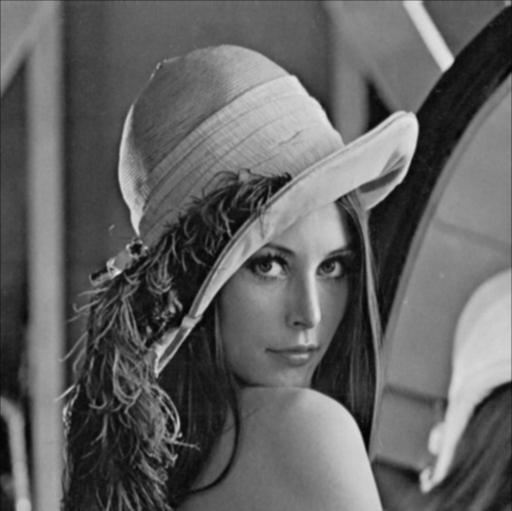
\includegraphics[scale=0.5]{lena_conv}
\\\\
(d)
Since Gaussian filter $F$ is separable, you can compute the horizontal and vertical filters, and perform a 1D convolution with the horizontal filter and image to each row followed by a 1D convolution with the vertical filter on each column. This is possible because of the associative property of convolution. You can verify the computed filters by finding the product of the horizontal and vertical filters is equal to the original Gaussian filter ($F=vh^T$). Separability allows for a faster filtering process since only 2 1D convolutions will need to be computed for every pixel in the image. This is illustrated in the following code with a faster convolution time of 0.001 s.
\begin{lstlisting}
im = imread('lena.png');

% create the Gaussian filter
sigma = 1;
filter = fspecial('gaussian', sigma * 3, sigma); 

% compute the vertical and horizontal filters of the Gaussian filter
[U,S,V] = svd(filter);
vertical_filter = sqrt(S(1,1)) * U(:,1);
horizontal_filter = sqrt(S(1,1)) * V(:,1)';

tic;
out = conv2(vertical_filter, horizontal_filter, im, 'same');
time_conv = toc;

imshow(out); % show the result of the convolution
fprintf('Time for convolution: %0.4f\n', time_conv);
% Time for convolution: 0.0010
\end{lstlisting}

%----------------------------------------------------------------
% Question 3
%----------------------------------------------------------------
\section{}
(a) Compute the magnitude of gradients for \textbf{waldo.png} and \textbf{template.png}.
\begin{lstlisting}
template = imread('template.png');
waldo = imread('waldo.png');

% compute the magnitude of gradients for the images
[template_grad_mag, template_grad_dir] = imgradient(rgb2gray(template));
[waldo_grad_mag, waldo_grad_dir] = imgradient(rgb2gray(waldo));

template_grad_mag = uint8(template_grad_mag);
waldo_grad_mag = uint8(waldo_grad_mag);

figure, imshow(template_grad_mag);
figure, imshow(waldo_grad_mag);
\end{lstlisting}
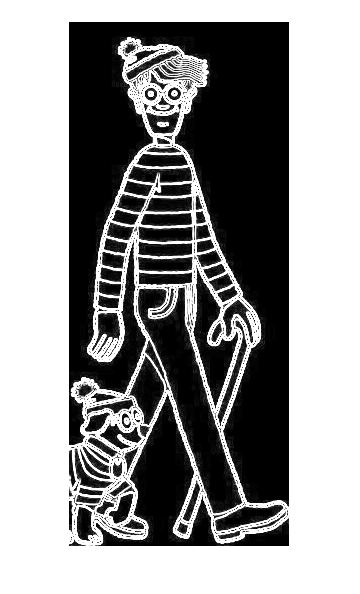
\includegraphics[scale=0.5]{templateGrad}
\\
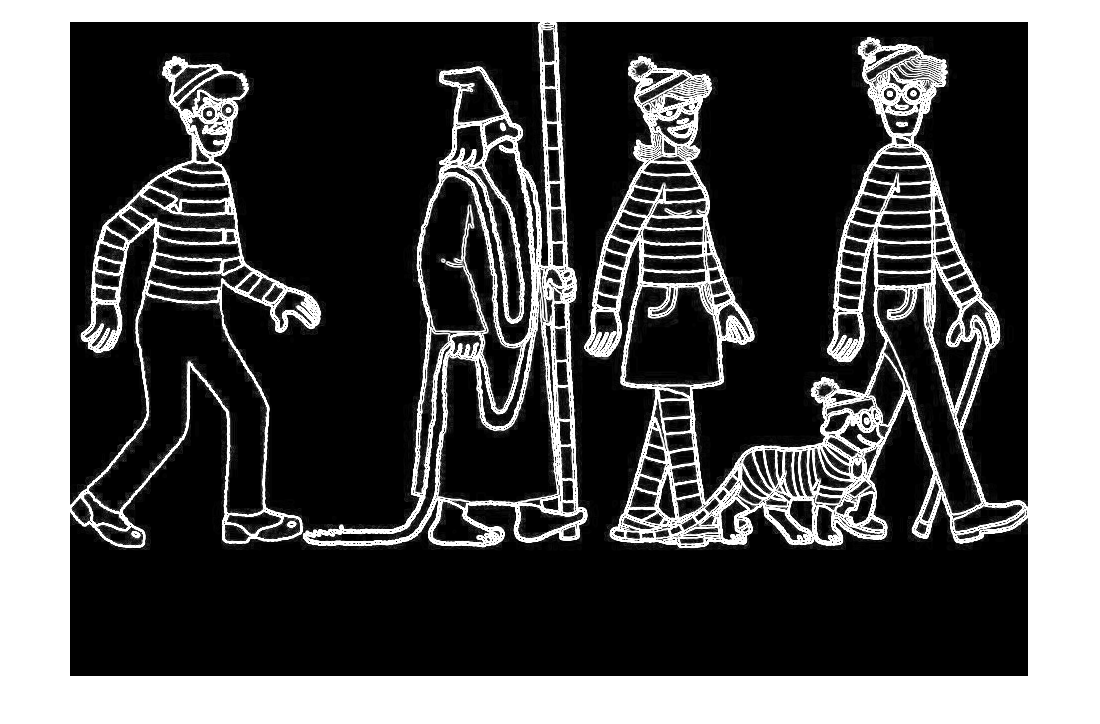
\includegraphics[scale=0.5]{waldoGrad}
\\
(b) Localize the template in the image \textbf{waldo.png} based on the magnitude of gradients.
\begin{lstlisting}
template = imread('template.png');
waldo = imread('waldo.png');

% compute the magnitude of gradients for the images
[template_grad_mag, template_grad_dir] = imgradient(rgb2gray(template));
[waldo_grad_mag, waldo_grad_dir] = imgradient(rgb2gray(waldo));

template_grad_mag = uint8(template_grad_mag);
waldo_grad_mag = uint8(waldo_grad_mag);

% Following code reused from lecture 2:
% normalized cross-correlation
out = normxcorr2(template_grad_mag, waldo_grad_mag);

% plot the cross-correlation results
figure('position', [100,100,size(out,2),size(out,1)]);
subplot('position',[0,0,1,1]);
imagesc(out)
axis off;
axis equal;

% find the peak in response
[y,x] = find(out == max(out(:)));
y = y(1) - size(template_grad_mag, 1) + 1;
x = x(1) - size(template_grad_mag, 2) + 1;

% plot the detection's bounding box
figure('position', [300,100,size(im,2),size(im,1)]);
subplot('position',[0,0,1,1]);
imshow(waldo)
axis off;
axis equal;
rectangle('position', [x,y,size(template_grad_mag,2),size(template_grad_mag,1)], 'edgecolor',
	[0.1,0.2,1], 'linewidth', 3.5);
\end{lstlisting}
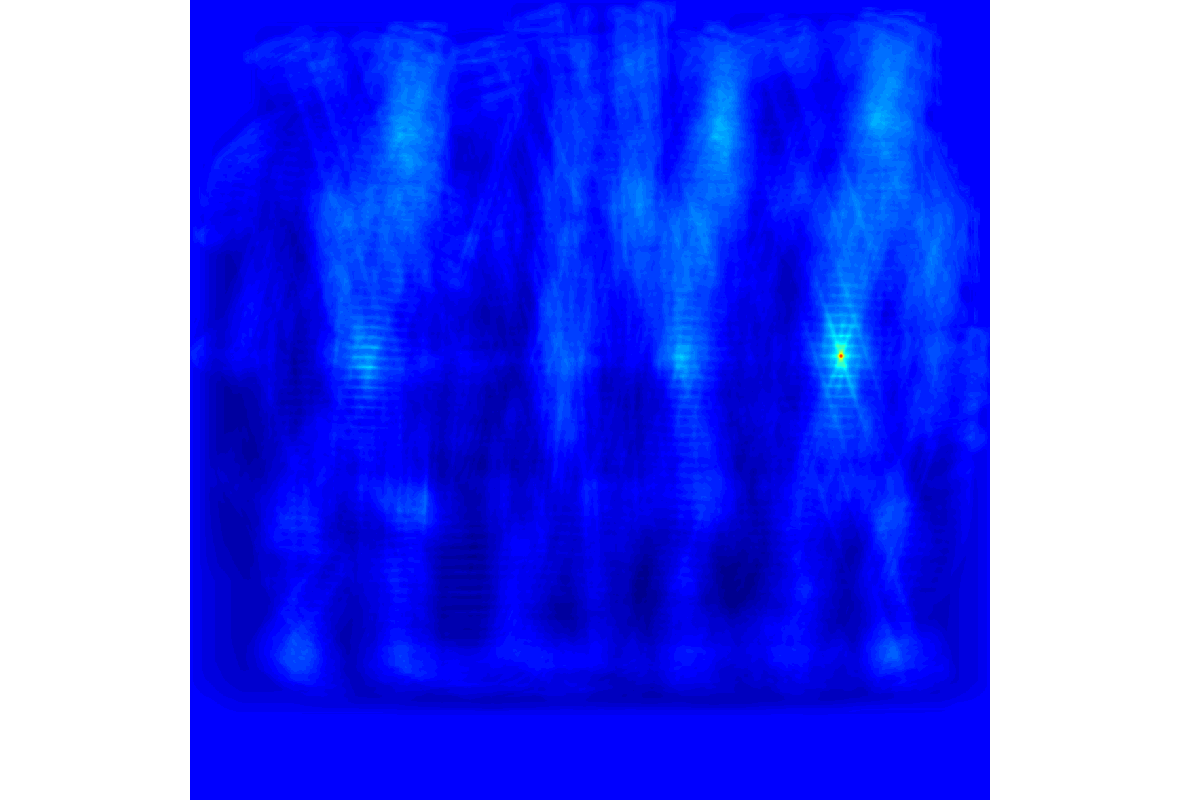
\includegraphics[scale=0.5]{normxcorrWaldo}
\clearpage
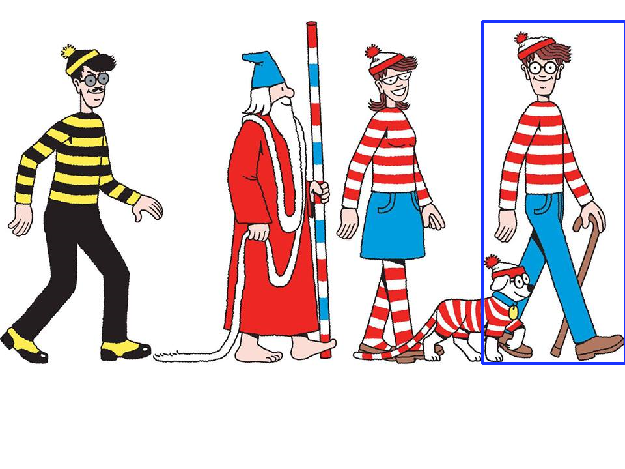
\includegraphics[scale=0.5]{waldoRect}
\\
(c) Compute the image pyramid with 3 levels for \textbf{waldo.png}.
\begin{lstlisting}
function out = impyramid(im)
% create the Gaussian filter
sigma = 1;
filter = fspecial('gaussian', sigma * 3, sigma);

% blur the image with the Gaussian filter
blur_im = imfilter(im, filter, 'same', 'conv');

% separate the channels of an RGB image
im_red = blur_im(:,:,1);
im_green = blur_im(:,:,2);
im_blue = blur_im(:,:,3);

% downsample the channels by a factor of 2
downsample_im_red = im_red(1:2:size(im_red,1), 1:2:size(im_red, 2));
downsample_im_green = im_green(1:2:size(im_green,1), 1:2:size(im_green, 2));
downsample_im_blue = im_blue(1:2:size(im_blue,1), 1:2:size(im_blue, 2));

% put the channels back together
out = cat(3, downsample_im_red, downsample_im_green, downsample_im_blue);
end

% compute the image pyramid with 3 levels for waldo.png
im = imread('waldo.png');
im1 = impyramid(im);
im2 = impyramid(im1);
im3 = impyramid(im2);

imshow(im);
figure, imshow(im1);
figure, imshow(im2);
figure, imshow(im3);
\end{lstlisting}
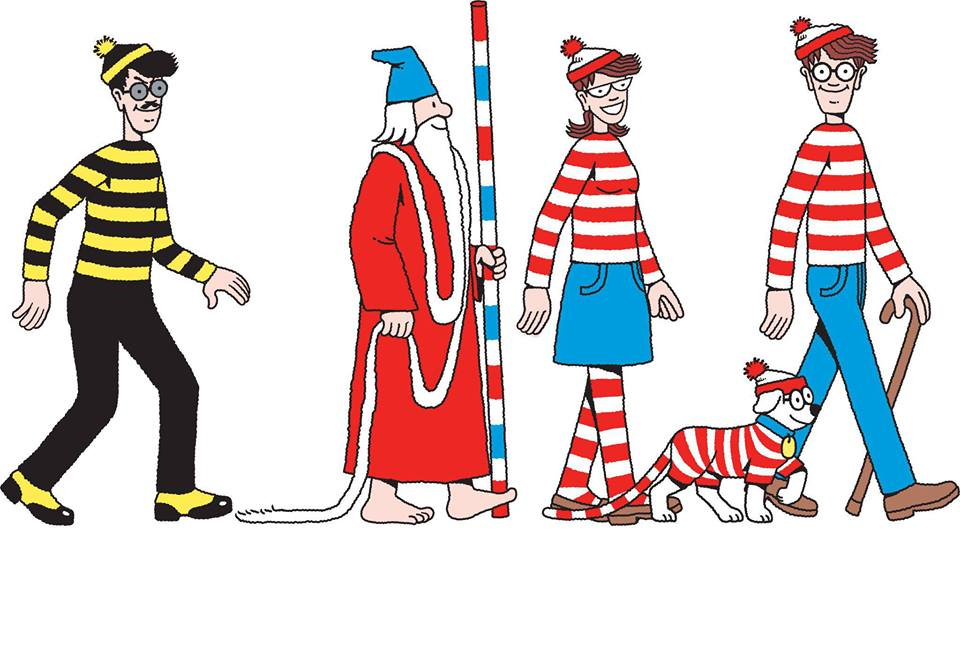
\includegraphics[scale=0.5]{waldo}
\\
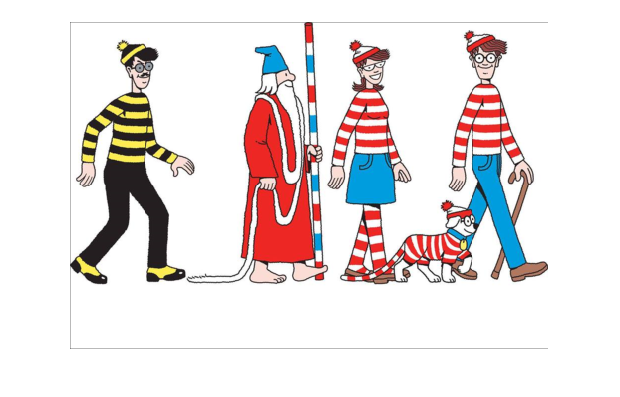
\includegraphics[scale=0.5]{waldoPy1}
\\
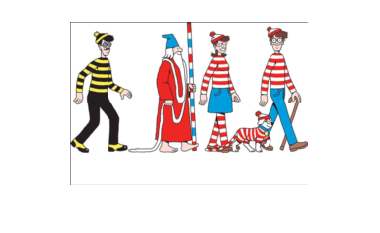
\includegraphics[scale=0.5]{waldoPy2}
\\
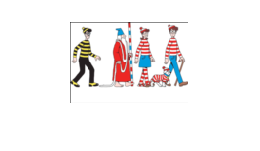
\includegraphics[scale=0.5]{waldoPy3}

%----------------------------------------------------------------
% Question 4
%----------------------------------------------------------------
\section{}
To reduce the amount of fine, detailed edges that are detected with the Canny edge detector, one can (1) raise the threshold of the low threshold, and (2) use a Gaussian filter with a larger $\sigma$.

%----------------------------------------------------------------
% Question 5
%----------------------------------------------------------------
\section{}
(a) Compute the magnitude of gradients for an image.
\begin{lstlisting}
im = imread('temple.jpg');

% compute the magnitude of gradients of the image
[imMag, imDir] = imgradient(rgb2gray(im));

imMag = uint8(imMag);

figure, imshow(im);
figure, imshow(imMag);
\end{lstlisting}
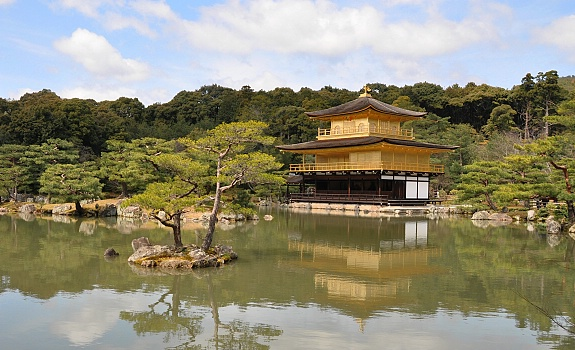
\includegraphics[scale=0.5]{temple}
\\
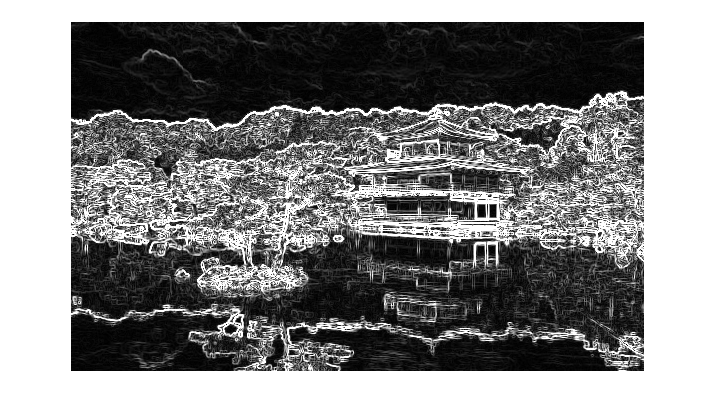
\includegraphics[scale=0.5]{templeGrad}
\end{document}